\documentclass[]{article}

\usepackage{fullpage}
\usepackage[colorlinks=true, linkcolor=blue, urlcolor=blue]{hyperref}
\usepackage{appendix}
\usepackage{pdfpages}
%opening
\title{Repurposing KwikByte FRC Driver Station}
\author{Carlos Gross Jones}

\begin{document}

\maketitle

\begin{abstract}

\end{abstract}

\section{Introduction}
\section{Dissection of Factory Image}
\par The first software item investigated was the image ``raw\_otb.bin'' provided by \href{http://www.kwikbyte.com/driverstation/binary/raw_otb.bin}{KwikByte} (also mirrored on \href{http://carlosgj.org/FRC/DS60/raw_otb.bin}{carlosgj.org} for posterity).
\par This file is not a first-level bootloader, but is instead called from the kernel loader. As such, it is expected to contain at least the Linux kernel and an initrd. In fact, the most recognizable thing in the file is the Linux boot parameters at offset 0x58:
\begin{verbatim}
console=ttyS0,115200 root=/dev/ram rw initrd=0x22400000,851719 mem=64M
\end{verbatim}
\par The purpose of the following data is unknown. However, an educated guess would be that a compressed Linux kernel exists in the file. Thus, the gzip ``magic number'', 0x1F8B, plus the expected compression method, 0x08, should be found (see the \href{https://tools.ietf.org/html/rfc1952}{gzip standard} for details). A search for 0x1F8B08 showed the first occurrence at offset 0x44F8. Metadata present in the gzip header reveals that the data was zipped on Fri, 03 Oct 2008 at 23:56:34 GMT on a Unix system. A partial copy of the raw\_otb.bin file from 0x44F8 to the end can indeed be unzipped, resulting in what appears to be a Linux kernel based on literal strings in the binary. In fact, one such string offers potentially valuable information:
\begin{verbatim}
Linux version 2.6.23DS60v1.0 (root@kbdev-laptop13) (gcc version 3.4.2) #7 
Fri Oct 3 16:56:31 MST 2008
\end{verbatim}
\par During the unzipping process, gzip noted that ``trailing garbage'' was ignored, indicating that the compressed archive beginning at 0x44F8 does not in fact extend to the end of the file. As the gzip standard specifies, the last four bytes of a member contain the size of the uncompressed data. Noting that the size of the unzipped kernel is 0x2BE6B0, this value was found in raw\_otb.bin at offset 0x160421, indicating the end of the first gzip archive. Shortly afterwards, at offset 0x160494, another occurrance of 0x1F8B08 is found, indicating the start of another archive. The metadata shows that it was zipped on Mon, 03 Nov 2008 at 20:23:39 GMT, with maximal compression, on a Unix system, and additionally that the original filename was ``initrd\_img''. Copying 0x160494 onwards results in another valid gzip, which successfully uncompresses into a filesystem. 
\newpage 
\begin{appendices}
	\section{Utility Loader \& Firmware Update Instructions}
		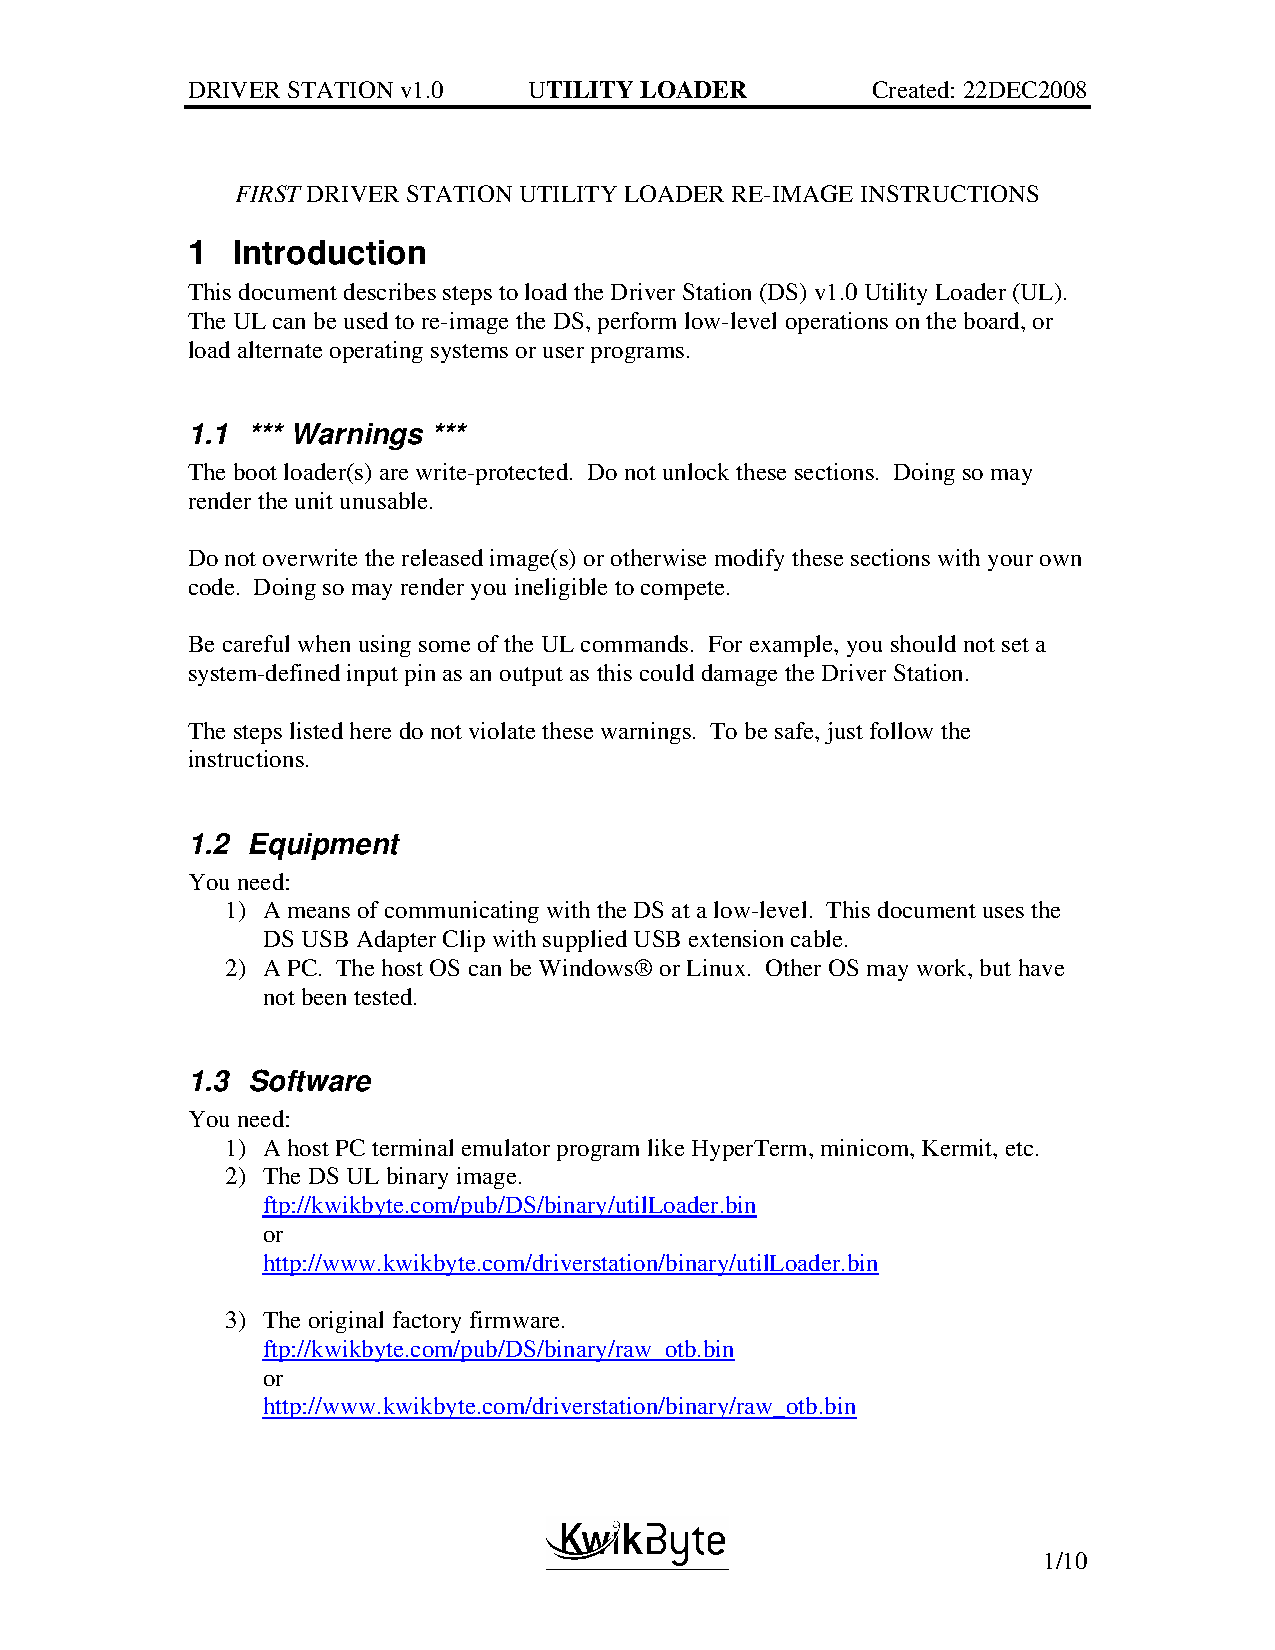
\includepdf[pages=-]{DS_utility_loader}
	\section{Kernel Loader Update Instructions}
		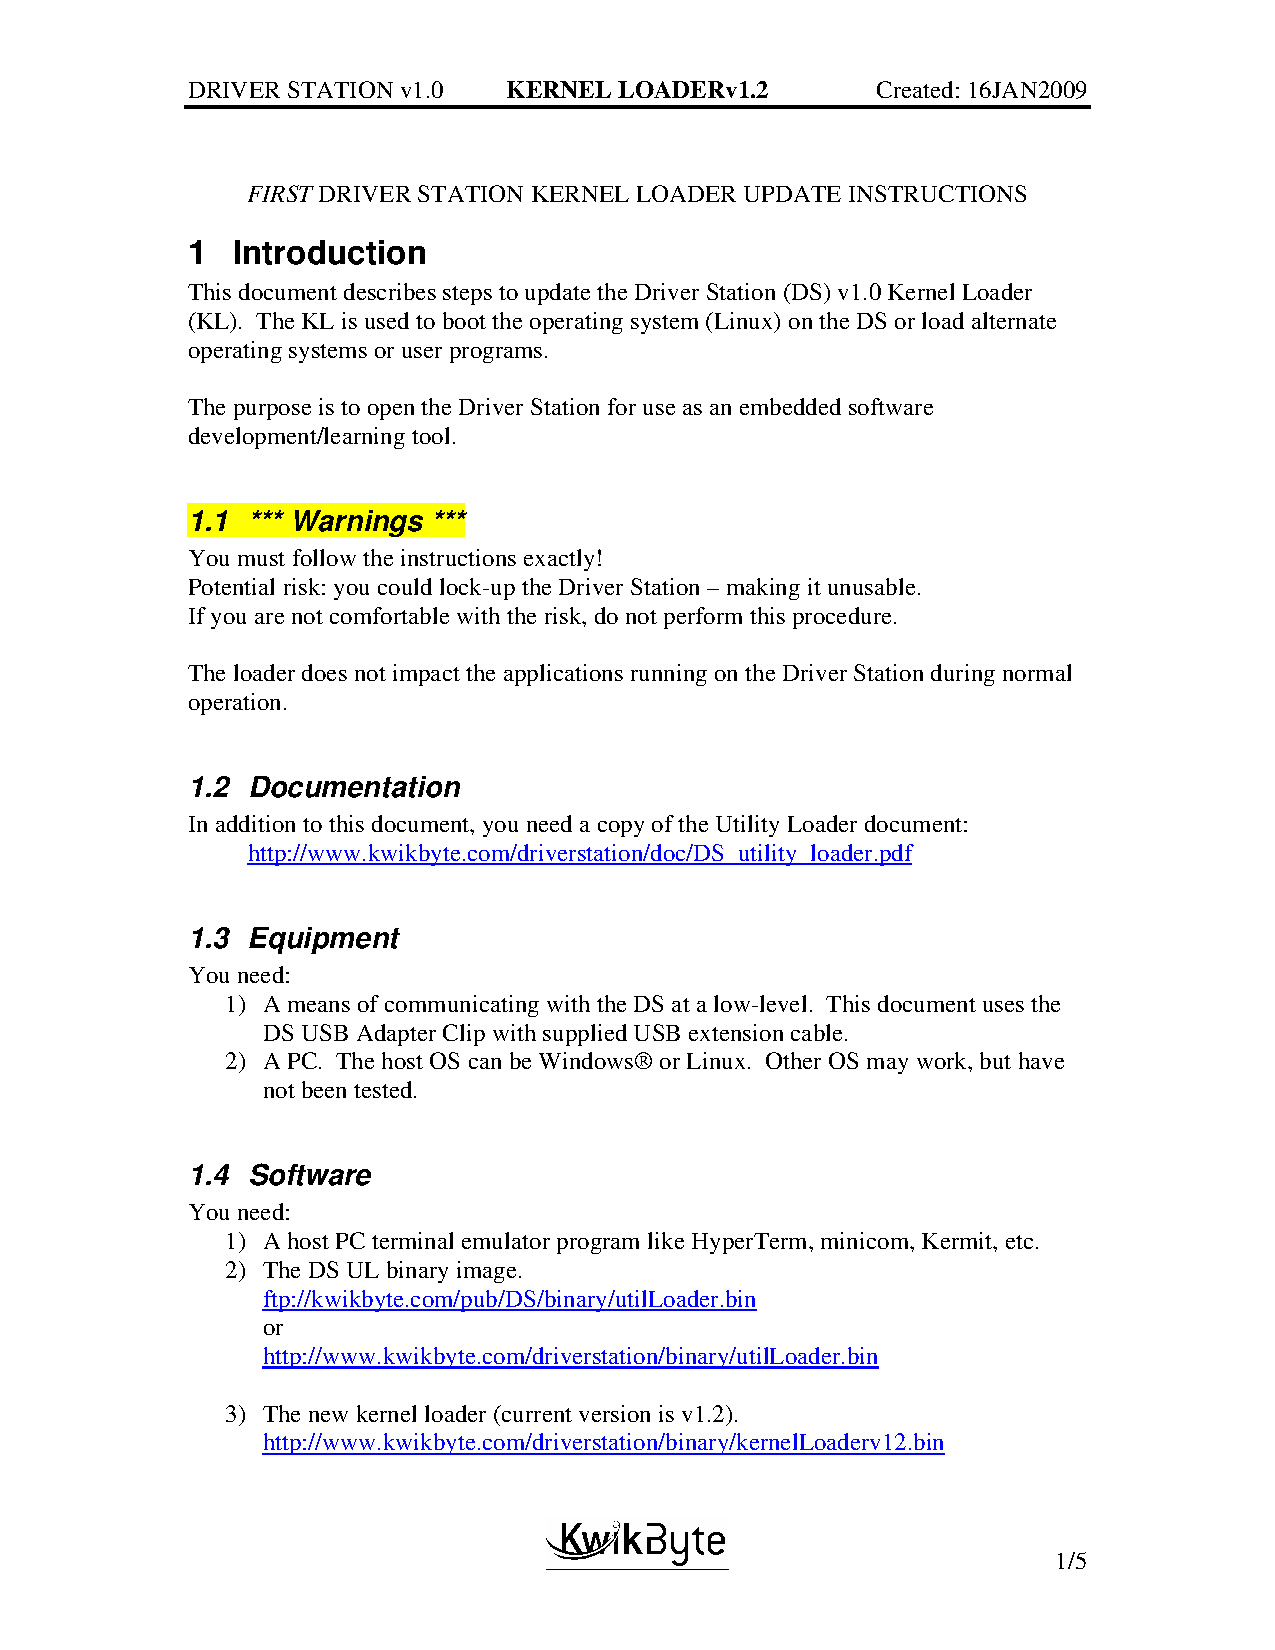
\includepdf[pages=-]{DS_kernelLoaderv12}
	\section{Logo Update Instructions}
		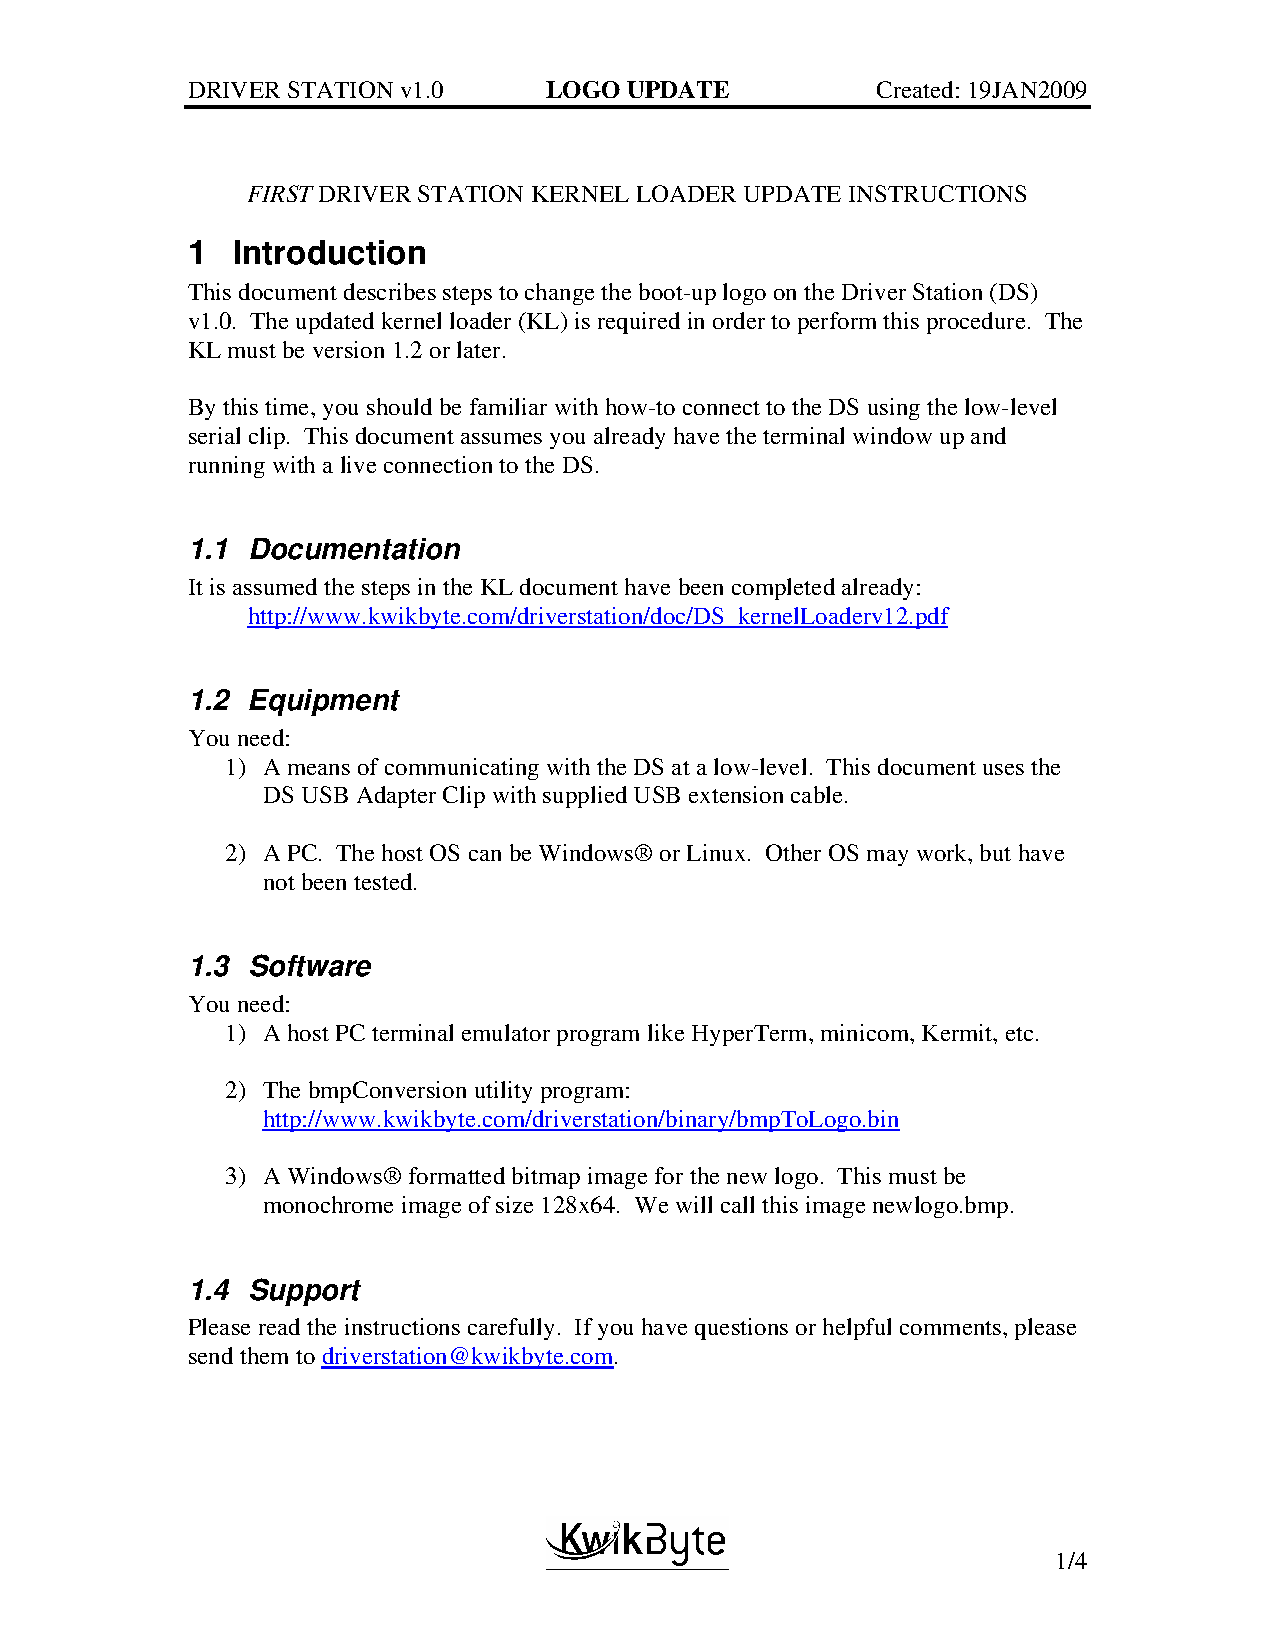
\includepdf[pages=-]{DS_logoUpdate}
\end{appendices}

\end{document}
